\chapter{Projektplan}
\section{Projektübersicht}
In diesem Projekt soll der Stand der Entwicklungen im Bereich \glqq Internet of Things\grqq{} aufgezeigt werden. Die verschiedenen Arten der eingesetzten Sensoren sollen ermittelt- und die Einsatzgebiete untersucht werden. Heutzutage werden in der Industrie bereits verschiedenartige Sensoren eingesetzt. Die Anzahl der eingesetzten Sensoren steigt drastisch. Schon bald stellt sich die Frage, wie man mit der steigenden Anzahl Sensoren deren Management realisieren soll.
\subsection{Zweck und Ziel}
Die Bachelorarbeit soll den Nachweis der Problemlösungsfähigkeit unter Anwendung
ingenieurmässiger Methoden nachweisen. Entsprechend verfügt die Arbeit über einen
konzeptionellen, theoretischen und einen praktischen Anteil.
\subsection{Projektorganisation}
\begin{table}[H]
\centering
    \begin{tabular}{@{} l l l@{}}    
    {Vorname} & {Name} & {E-Mail} \\ \midrule
    Andreas & Stalder & astalder@hsr.ch \\ \addlinespace
    David & Meister & dmeister@hsr.ch \\ \bottomrule
    \end{tabular}
\end{table} 

Das Projekt wird von Prof. Beat Stettler und Urs Baumann betreut und benotet.
\section{Management Abläufe}
\subsection{Zeitbudget}
Der Projektstart ist am Montag, dem 20. Februar 2017. \\
Die Projektdauer beträgt 17 Wochen, und das Projektende ist am Freitag, dem 16. Juni 2017. \\

\noindent Während diesen 17 Wochen sind 360 Arbeitsstunden pro Projektmitglied eingeplant. Das entspricht pro Mitglied eine Arbeitszeit von ca. 22 Stunden pro Woche. Dies ergibt einen totalen Aufwand von ca. 720 Stunden.\\

\noindent Die wöchentliche Arbeitszeit von 22 Stunden kann bei Verzug oder bei unerwarteten Problemen auf maximal 30 Stunden erhöht werden. \\

\noindent Es sind gegenwärtig keine Absenzen während dieser Zeit geplant.

\subsection{Projektphasen}
Das Projekt wird in fünf Phasen unterteilt: Initialisierung, Analyse, Design, Realisierung und Abschluss.
\newline
\begin{figure}[H]
\centering
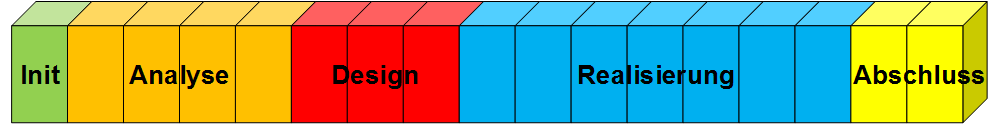
\includegraphics[width=1\textwidth]{../01_Projektplanung/images/phasen.png}
\caption{Projektphasen}
\end{figure}
\subsection{Meilensteine}
Das Projekt beinhaltet insgesamt vier Meilensteine. \\
\begin{table}[H]
    \begin{tabular}{@{} l l l r@{}}\toprule    
    {Meilenstein} & {Beschreibung} & {Datum}\\ \midrule
    MS1 & Anforderungen und Scope definiert  & 26.03.2017\\ \addlinespace
    MS2 & Architektur und Design beschrieben & 23.04.2017\\ \addlinespace
    MS3 & Software fertiggestellt, Codefreeze  & 04.06.2017\\ \addlinespace
    MS4 & Arbeitsabgabe & 16.06.2017\\ 
    \bottomrule
    \end{tabular}
\caption{\textbf{Projekt Meilensteine}}
\end{table}
\newpage
\subsection{Iterationen}
Die Dauer eines Iterationszyklus beträgt jeweils eine Woche. 
\begin{table}[htb]
\centering
    \begin{tabular}{@{} p{3cm} l l l@{}}\toprule    
    {Iteration} & {Inhalt} & {Start} & {Ende}\\ \midrule
    Initialisierung 1 & Kickoff Meeting, Projektplanung, Infrastruktur & 20.02.2017 & 26.02.2017\\ \addlinespace
    Analyse 1 & IoT-Analyse Allgemein & 27.02.2017 & 05.03.2017\\ \addlinespace
    Analyse 2 & IoT-Analyse Allgemein & 06.03.2017 & 12.03.2017\\ \addlinespace
    Analyse 3 & Sensoren Analyse technisch \& Evaluation & 13.03.2017 & 19.03.2017\\ \addlinespace
    Analyse 4 & Requirements definieren & 20.03.2017 & 26.03.2017\\ \addlinespace
    Design 1 & Architektur beschreiben, Risikoanalyse & 27.03.2017 & 02.04.2017\\ \addlinespace
    Design 2 & Prototyp programmieren & 03.04.2017  & 09.04.2017\\ \addlinespace
    Design 3 & Prototyp programmieren & 10.04.2017  & 16.04.2017\\ \addlinespace
    Design 4 & Requirements- und Architektur Review & 17.04.2017  & 23.04.2017\\ \addlinespace
    Realisierung 1 & Implementation & 24.04.2017  & 30.04.2017\\ \addlinespace
    Realisierung 2 & Implementation & 01.05.2017  & 07.05.2017\\ \addlinespace
    Realisierung 3 & Implementation & 08.05.2017  & 14.05.2017\\ \addlinespace
    Realisierung 4 & Implementation & 15.05.2017  & 21.05.2017\\ \addlinespace
    Realisierung 5 & Implementation & 22.05.2017  & 28.05.2017\\ \addlinespace
    Realisierung 6 & Refactoring / Bugfixing & 29.05.2017  & 04.06.2017\\ \addlinespace
    Abschluss 1 & Dokumentation &  05.06.2017 & 11.06.2017\\ \addlinespace
    Abschluss 2 & Dokumentation &  12.06.2017 & 16.06.2017\\ \addlinespace
    \bottomrule
    \end{tabular}
\caption{\textbf{Projekt Iterationen}}
\end{table}

\begin{landscape}
\subsection{Arbeitspakete}
\begin{longtable}{ p{5.5cm} p{8cm} l l p{1cm} p{1cm} }

\hline 
\multicolumn{1}{p{5.5cm}}{\textbf{Name}} & \multicolumn{1}{p{8cm}}{\textbf{Inhalt}} & \multicolumn{1}{l}{\textbf{Iteration}} & \multicolumn{1}{l}{\textbf{Wer}} & \multicolumn{1}{p{1cm}}{\textbf{Soll}} & \multicolumn{1}{p{1cm}}{\textbf{Ist}} \\ \hline 
\endfirsthead

\hline 
\multicolumn{1}{p{5.5cm}}{\textbf{Name}} & \multicolumn{1}{p{8cm}}{\textbf{Inhalt}} & \multicolumn{1}{l}{\textbf{Iteration}} & \multicolumn{1}{l}{\textbf{Wer}} & \multicolumn{1}{p{1cm}}{\textbf{Soll}} & \multicolumn{1}{p{1cm}}{\textbf{Ist}} \\ \hline 
\endhead

\textbf{Initialisierung}&&&&\\ \addlinespace
Kickoff-Meeting & Allgemeine Besprechungen zum Projektstart & Initialisierung 1 & Alle & 1 & 1 \\ \addlinespace
Dokumenterstellung & Erstellung \LaTeX{} Vorlagen & Initialisierung 1 & Alle & 4 & 5 \\ \addlinespace
Projektplan & Zeitplanung, Phasen, Meilensteine & Initialisierung 1 & Alle & 5 & 6 \\ \addlinespace
Einrichtung Projektmanagement Software & Installation und Einrichtung Jira & Initialisierung 1 & Alle & 3 & 5 \\ \addlinespace

\textbf{Analyse}&&&&\\ \addlinespace
Einarbeitung IoT-Allgemein & IoT-Übersicht erarbeiten und dokumentieren & Analyse 1/2 & dm & 25 & 32\\ \addlinespace
Einarbeitung Sensortypen & Sensortypen recherchieren und dokumentieren & Analyse 1/2 & as & 15 & 12\\ \addlinespace
Einarbeitung Kommunikation & IoT-relevante Kommunikationsbereiche analysieren und dokumentieren & Analyse 1/2 & Alle & 40 & 44\\ \addlinespace
Einarbeitung Management & Device Management in IoT & Analyse 3 & Alle & 40 & 52\\ \addlinespace
Requirements & Funktionale Anforderungen (Use Cases) und Nichtfunktionale Anforderungen & Analyse 4 & Alle & 40 & 29\\ \addlinespace


\textbf{Design}&&&&\\ \addlinespace
Architekturübersicht & Übersichtsverschaffung, Grobkonzept & Design 1 & dm & 8 & 6\\ \addlinespace
Domain Model & Erstellung des Domänenmodells & Design 1 & Alle & 8 & 8\\ \addlinespace
Schichtenarchitektur & Erstellung der Schichtenarchitektur, Packages schnüren & Design 1 & as & 8 & 6\\ \addlinespace
Auswahl Frameworks & Frameworks für Front- \& Backend sowie Datenbank analysieren und auswählen & Design 1-4 & Alle & 60 & 76\\ \addlinespace
Prototyp & Erstellung eines Prototypen über alle Softwareschichten & Design 2-4 & Alle & 90 & 128\\ \addlinespace

\textbf{Realisierung}&&&&\\ \addlinespace
Anpassungen Architektur  & Anpassungen Architektur gem. Reviews & Realisierung 1 & Alle & 30 & 22\\ \addlinespace
Erstellung Views  & Seitenaufbau mit verschiedenen Views aufgebaut & Realisierung 1 & Alle & 10 & 14\\ \addlinespace
Gruppenverwaltung implementieren & Navigationsbaum, Gruppen CRUD etc. & Realisierung 2-4 & Alle & 53 & 58\\ \addlinespace
Deviceverwaltung implementieren & Anzeige, Kommunikation & Realisierung 2-4 & Alle & 47 & 37\\ \addlinespace
Discovery implementieren & Implementieren Device Discovery & Realisierung 3, 5 & Alle & 14 & 16\\ \addlinespace
Konfigurationsverwaltung implementieren & Implementieren Konfigurationsverwaltung & Realisierung 4-5 & Alle & 27 & 26\\ \addlinespace
Login + User Management implementieren & Login + User Management implementieren implementieren & Realisierung 5 & Alle & 10 & 13\\ \addlinespace
Dashboard implementieren & Login + User Management implementieren implementieren & Realisierung 5-6 & Alle & 18 & 19\\ \addlinespace
Devicemap implementieren & Implementierung Google Map & Realisierung 5 & Alle & 4 & 6\\ \addlinespace
Testing & Integrationstests & Realisierung 6, Abschluss 1 & Alle & 16 & 15\\ \addlinespace
Refactoring & Struktur- und Codeanpassungen & Realisierung 6, Abschluss 1 & Alle & 32 & 36\\ \addlinespace
Bugfixing & Beheben von Softwarefehlern & Realisierung 6 & Alle & 8 & 18\\ \addlinespace
Testclient aufsetzen & LwM2M Testclient aufbauen & Realisierung 6 & Alle & 4 & 5\\ \addlinespace

\textbf{Abschluss}&&&&\\ \addlinespace
Schlussbericht erstellen & Schlussbericht erstellen und abgeben & Abschluss 1-2 & Alle & 100 & 138\\ \addlinespace
Anleitungen erstellen & Benutzer- und Installationsanleitung erstellen & Abschluss 2 & Alle & 12 & 9\\ \addlinespace


\addlinespace


\hline\caption{\textbf{Arbeitspakete}}
\end{longtable}
\end{landscape}

\subsection{Teammeetings}
Besprechungen finden dreimal wöchentlich jeweils an den vorgesehenen Arbeitstagen statt. 
Besprechungen dauern in der Regel 10-15 Minuten. Es wird das weitere Vorgehen, sowie durchgeführte Arbeiten, fällige Arbeiten und auftretende Probleme besprochen. Weiter werden Arbeitspakete verteilt, damit beide Projektmitglieder wissen was zu tun ist. 

\subsection{Meeting mit Betreuern}
Die Meetings mit den Betreuern finden jeden Freitag um 14:00 Uhr statt. 
Die Meetings werden mit den Betreuern Prof. Beat Stettler und Urs Baumann in ihrem Büro durchgeführt. Die Meetings dauern normalerweise zwischen 30-60 Minuten. 

\section{Qualitätsmassnahmen}
\subsection{Versionierung}
Wie die Dokumentation wird auch der Sourcecode mit git versioniert und auf GitHub abgelegt. Es wird darauf geachtet, möglichst häufig auf den Stamm zu commiten.
\subsection{Reviews}
Regelmässige Reviews sind in einem iterativen Vorgehen unerlässlich. Die getätigte Arbeit muss ständig abgeglichen und in Frage gestellt werden. Aus Kosten-Nutzen Sicht sind Reviews das effektivste Mittel um die geforderte Qualität zu erreichen.\\ 

\noindent In diesem Projekt werden drei verschiedene Arten von Reviews durchgeführt. Zum einen sind dies regelmässige Code Reviews, zum anderen sind dies Requirement- und Architekturreviews.\\

\noindent Bei den regelmässigen Code Reviews wird besonders auf die gewählten Namen (Packages, Klassen, Methoden, Variablen), die Verständlichkeit vom Code und Code Smells geachtet.\\

\noindent Bei den Requirement Reviews wird sichergestellt, dass man den Wünschen des Auftraggebers entsprechend entwickelt. Die Frage nach dem \glqq Was\grqq{} wird erneut gestellt und somit sichergestellt, dass man beim Projektende nicht ein qualitativ hochwertiges Produkt entwickelt hat, welches aber nicht die Wünsche des Auftraggebers abdeckt.\\ 

\noindent Beim Architektur Review wird besonders auf die nicht-funktionalen Anforderungen (NFA) geachtet. Diese wirken sich in den meisten Fällen auf die gewählte Architektur aus. Die gewählte Architektur muss mit den NFAs verträglich sein. Wenn zu spät im Projekt bemerkt wird, dass die Architektur geändert werden muss, kann dies sehr aufwändig sein.
\subsection{Code Metriken}
Code Metriken zeigen mögliche Fehler oder Schwachstellen im entwickelten Code auf. Es wird grundsätzlich zwischen statischen- und dynamischen Metrik Tools unterschieden. Bei den dynamischen Metrik Tools wird der Code ausgeführt. Beispiele wären Unit Tests und die dazugehörige Coverage. Bei den statischen Analysetools wird der Code nicht ausgeführt. Ein Beispiel wäre Checkstyle. Dieses Tool überprüft vor allem die Einhaltung von Style Richtlinien.\\